\documentclass[12pt, twoside]{article}
\usepackage[letterpaper, margin=1in, headsep=0.2in]{geometry}
\setlength{\headheight}{0.6in}
%\usepackage[english]{babel}
\usepackage[utf8]{inputenc}
\usepackage{microtype}
\usepackage{amsmath}
\usepackage{amssymb}
%\usepackage{amsfonts}
\usepackage{siunitx} %units in math. eg 20\milli\meter
\usepackage{yhmath} % for arcs, overparenth command
\usepackage{tikz} %graphics
\usetikzlibrary{quotes, angles}
\usepackage{graphicx} %consider setting \graphicspath{{images/}}
\usepackage{parskip} %no paragraph indent
\usepackage{enumitem}
\usepackage{multicol}
\usepackage{venndiagram}

\usepackage{fancyhdr}
\pagestyle{fancy}
\fancyhf{}
\renewcommand{\headrulewidth}{0pt} % disable the underline of the header
\raggedbottom
\hfuzz=2mm %suppresses overfull box warnings

\usepackage{hyperref}
\usepackage[nomessages]{fp}% http://ctan.org/pkg/fp

\fancyhead[LE]{\thepage}
\fancyhead[RO]{\thepage \\ Name: \hspace{4cm} \,\\}
\fancyhead[LO]{BECA / Dr. Huson / Geometry\\*  Unit 1: Segments, length, and area\\* 21 Sept 2022}

\begin{document}

\subsubsection*{1.10 Extension: Confidence intervals and the margin of error}
\emph{Learn to use and intepret common notation for confidence intervals} (see \href{https://www.mathbootcamps.com/three-ways-write-confidence-interval/}{MathBootCamps})
\begin{itemize}
    \item Plus or minus a \emph{margin of error}. e.g. $v = 24.8 \pm 4.5$
    \item As an interval or range, $(20.3, 29.3)$. (brackets are also used, i.e. $[20.3, 29.3]$)
    \item As an inequality, $20.3 \leq v \leq 29.3$
\end{itemize} \vspace{1cm}

\begin{enumerate}
\item The height of a Christmas tree rounded to the nearest foot is 7 feet. What is the shortest the tree could be? The tallest? Express your answer as an interval or range, with parenthesis. \vspace{1cm}

\item Express the value $v=10 \pm 1.5$ as an inequality. \vspace{1cm}

\item A person's weight is estimated as 125 lbs. plus or minus 5 lbs. Express that as a percent, i.e. in the form $125 \pm x\%$. \vspace{2cm}

\item The radius of a circle rounded to the nearest foot is 10 feet. Find the possible values for the area of the circle. Express your answer as an interval / range. \vspace{3cm}

\item The length of a rectangular field is between 20 and 21 meters, and its width is between 8 and 9 meters. Find the area of the field, expressed as an inequality.

\newpage
%\usepackage[nomessages]{fp}
    \FPeval{\inscr}{round(0.5*10*sin(36*pi/180),4)} 
        %Inscribed area: $\inscr$ \par
    \FPeval{\mul}{1/cos(18*pi/180)}
        %Cos inv multiplier: $\mul$ \par
    \FPeval{\circum}{round(\inscr * \mul * \mul,4)} 
        %Circumscribed area: $\circum$ \par
\item The diagram shows a circle sandwiched between two decagons (10-sided polygons). The area of the smaller, inscribed decagon is $A_{inner} \approx \inscr$ and the larger, circumscribed decagon's area is $A_{outer} \approx \circum$. Use these bounds to approximate $\pi$ plus or minus a margin of error.
\par

  \begin{tikzpicture}[scale=1, rotate=18]
    \draw[thick] (0,0) circle[radius=3];
    \draw (0:3)--(36:3)--(2*36:3)--
    (3*36:3)--(4*36:3)--(5*36:3)--(6*36:3)--(7*36:3)--(8*36:3)--(9*36:3)--cycle;
    \fill (0,0) circle[radius=0.08];
    \draw[<->,thick](0.1,0)--(2.95,0);
    \draw (1.7,0) node[below]{$1$};
    \draw[scale=1.0515, rotate=18] (0:3)--(36:3)--(2*36:3)--
    (3*36:3)--(4*36:3)--(5*36:3)--(6*36:3)--(7*36:3)--(8*36:3)--(9*36:3)--cycle;
  \end{tikzpicture}
    
\item Find the area of the $\triangle ABC$ is shown below with $A(3,2)$, $B(7,4)$, and $C(4,8)$. 
  \begin{multicols}{2}
    \begin{enumerate}
      \item First find the area of the red rectangle with sides $b=4$, $h=6$.
      \item Find the area of the three triangles surrounding $\triangle ABC$ in the rectangle. 
      \item Subtract their areas from the rectangle to find $A_{\triangle ABC}$
      \end{enumerate}
      \begin{flushright}
      \begin{tikzpicture}[scale=.635]
        \draw[help lines] (-1,-1) grid (9,9);
        \draw[thick, ->] (-1.2,0) -- (9.4,0) node [below right] {$x$};
        \draw[thick, ->] (0,-1.2)--(0,9.4) node [left] {$y$};
        \draw[thick] (3,2)--(7,4)--(4,8)--cycle;
        \draw[thick, red] (3,2)--(7,2)--(7,8)--(3,8)--cycle;
        \draw[fill] (3,2) circle [radius=0.05] node[below left] {$A$};
        \draw[fill] (7,4) circle [radius=0.05] node[right] {$B$};
        \draw[fill] (4,8) circle [radius=0.05] node[above right] {$C$};
        \node at (5,2)[below]{$4$};
        \node at (2.2,5)[right]{$6$};
      \end{tikzpicture}
      \end{flushright}
  \end{multicols}


\end{enumerate}
\end{document}